% Document template based on LNCS, adapted by Matt Welsh <mdw@cs.berkeley.edu>

% This version is adapted to use PDFTEX to render to PDF directly. 
% If you want to use dvi, you need to change any figures to use '.eps'
% rather than '.pdf', and probably get rid of the hyperref package.

\documentclass{article}
%\usepackage{program}
\usepackage{acm-style10} % ACM proceedings formatting
\usepackage{times}  % Use Adobe Times font set
\usepackage{epsfig,twocolumn}
\usepackage{url}
\usepackage[english]{babel} % mdw: Required to get good hyphenation on RH6.0
                            % (fixed in RH6.1)
\usepackage{graphicx} 
\usepackage{color}     % This will generate links within the PDF as well as a set of bookmarks
\usepackage{amsmath}   % For the theory section (added by RADHIKA)
% \usepackage[colorlinks,pdfpagemode=None]{hyperref} 

%\def\dsp{\def\baselinestretch{0.92}\large\normalsize}
%\def\dsp{\def\baselinestretch{0.92}}
%\dsp
\def\dsp{\def\baselinestretch{1.05}}
\dsp

\newcommand{\XXXnote}[1]{{\textcolor{red}{\bf XXX: #1}}}

%set dimensions of columns, gap between columns, and space between
%paragraphs
\setlength{\textheight}{9.75in}
\setlength{\columnsep}{0.25in}
\setlength{\textwidth}{7.5in}
\setlength{\footskip}{0.0in}
\setlength{\topmargin}{-0.5in}
\setlength{\headheight}{0.0in}
\setlength{\headsep}{0.0in}
%\setlength{\oddsidemargin}{-.45in}
\setlength{\oddsidemargin}{-0.5in}
\setlength{\parindent}{1pc}
%\setlength{\parskip}{\baselineskip}

%\setlength{\textheight}{9.25in}
%\setlength{\columnsep}{0.33in}
%\setlength{\textwidth}{7.4in}
%\setlength{\footskip}{0.0in}
%\setlength{\topmargin}{-0.25in}
%\setlength{\headheight}{0.0in}
%\setlength{\headsep}{0.0in}
%\setlength{\oddsidemargin}{-.45in}
%%\setlength{\oddsidemargin}{0in}
%\setlength{\parindent}{1pc}
%%\setlength{\parskip}{\baselineskip}


% Define a command for putting in figures:
% Use as follows:
% \pic{sizeparams}{filename}{caption}{label}
% Example: \pic{width=3in}{./figures/mypic.pdf}{\small Caption text}{fig-myfig}

\newcommand{\pic}[5][ht]{
\begin{figure}[t] %[t]
\begin{center}
\includegraphics[keepaspectratio,#2]{#3}
\end{center}
\caption{#4}
\label{#5}
\end{figure}
}

\pagestyle{empty}
\begin{document}

%don't want date printed
\date{}

%%%%%%%%%%%% THIS IS WHERE WE PUT IN THE TITLE AND AUTHORS %%%%%%%%%%%%

\title{{\ttlfnt Firefly-Inspired 
Sensor Network Synchronicity with Realistic Radio Effects}}


%\author{{\aufnt } \\
%{\aufnt } \\
%{\affaddr Division of Engineering and Applied Sciences} \\
%{\affaddr Harvard University} \\
%{\affaddr \{werner,gtewari,abpatel,mdw,rad\}@eecs.harvard.edu}} 

\maketitle
%\copyrightspace

\thispagestyle{empty}

%%%%%%%%%%%%%  SKELETON OF THE PAPER   %%%%%%%%%%%%%%

%% 1. Abstract [ALL, DUE TOMORROW]

%% 2. Introduction [MATT/RAD]
%%    - why synchronicity is important
%%    - synchronicity in biology 

%% 3. Related Work [MATT]
%%    - attempts to implement in ad-hoc networks
%%    - other time sync protocols?
   
%% 4. Firefly inspired Synchronization Algorithm [RAD]
%%    - Mirollo and Strogatz model
%%    - Differences between theory and practice
%%    - Our Modified Firefly-inspired Algorithm

%% 5. Theoretical Results [ANKIT]
%%    - Proof of convergence for n=2
%%    - Proof of relation between convergence rate and epsilon
%%    - Intuition about choice of epsilon

%% 6. Simulation Results [GEETIKA]
%%    - explanation of what TOSSIM models and what it does not (justify)
%%      especially with regards to radio model.
%%    - Scatter plot of phase vs time for one example
%%    - Time to sync and Group Spread for
%%       - all-to-all, varying n and epsilon
%%       - grid, varying nxn and epsilon
%%       - mote deployment topology, and epsilon
%%    - Discussion of how well the data matches the theory.

%% 7. Motelab Results [GWA]
%%    - explanation of setup and use of FTSP to timestamp
%%    - For a given (good) epsilon choice
%%        - Graph of Phase vs time
%%        - Distribution of Phase offsets 
%%          (perhaps broken down by number of hops)

%% 8. Discussion [ALL]
%% 9. Bibliography

%%%%%%%%%%%%%  BODY OF PAPER GOES HERE %%%%%%%%%%%%%%

%\section{Introduction}

Computer scientists have often looked to nature for inspiration.
Researchers studying distributed systems have long envied, and
attempted to duplicate, the fault-tolerance and decentralized control
achieved in natural systems.  Those of us studying sensor networks
also have every reason to be envious.  Designing software coordinating
the output of a collection of limited devices frequently feels as
frustrating as orchestrating the activity of a colony of stubborn
ants, or guiding a school of uncooperative fish.  And yet ant colonies
complete difficult tasks, schools of fish navigate the sea, and swarms
of fireflies stretching for miles can pulse in perfect unison, all
without centralized control or perfect individuals. The spontaneous
emergence of synchronicity --- for example, fireflies flashing in
unison or cardiac cells firing in synchrony --- has long attracted the
attention of biologists, mathematicians and computer scientists.

%% SIMULTANEOUS COLLECTIVE ACTION

Synchronicity is a powerful primitive for sensor networks. We define
synchronicity as the ability to organize {\em simultaneous collective
action} across a sensor network. Synchronicity is not the same as time
synchronization: the latter implies that nodes share a common notion
of time that can be mapped back onto a real-world clock, while the
former only requires that nodes agree on a firing period and phase.
The two primitives are complementary: nodes with access to a common
time base can schedule collective action in the future, and
conversely, nodes that can arrange collective action can establish a
meaningful network-wide time base. However, the two primitives are also
independently useful. For example, nodes within a sensor network may
want to compare the times at which they detected some event. This task
requires a notion of global time, however it does not require
real-time coordination of actions. 

Similarly, synchronicity by itself can be extremely useful as a sensor
network coordination primitive. A commonly-used mechanism for limiting
energy use is to carefully schedule node duty cycles so that all nodes
in a network (or a portion of the network) will wake up at the same
time, sample their sensors, and relay data along a routing path to the
base station. Coordinated communication scheduling has been used both
at the MAC level~\cite{s-mac} and in multi-hop routing
protocols~\cite{stem} to save energy. Synchronicity can also be
used to coordinate sampling across multiple nodes in a network,
which is especially important in applications with high data
rates. Previous work on seismic analysis of
structures~\cite{glaser-smart-buildings}, shooter
localization~\cite{shooter-localization}, and volcanic
monitoring~\cite{volcano-ewsn05} could use such a primitive and avoid
the overhead of maintaining consensus on global time until
absolutely necessary.

In this paper, we present a biologically-inspired distributed
synchronicity algorithm implemented on TinyOS motes. This algorithm is
based on a mathematical model originally proposed by Mirollo and
Strogatz to explain how neurons and fireflies spontaneously
synchronize~\cite{strogatz}. This seminal work proved that a very
simple reactive node behavior would always converge to produce global
synchronicity, irrespective of the number of nodes and starting
times. Recently Lucarelli and Wang~\cite{lucarelli04} demonstrated
that this result also holds for multi-hop topologies, an important
contribution towards making the model feasible for sensor networks.

The firefly-inspired synchronization described by Mirollo and Strogatz
has several salient features that make it attractive for sensor
networks. Nodes execute very simple computations and interactions, and
maintain no internal state regarding neighbors or network topology. As
a result, the algorithm robustly adapts to changes such as the loss
and addition of nodes and links \cite{lucarelli04}. The synchronicity
provably emerges in a completely decentralized manner, without any
explicit leaders and irrespective of the starting state.

However, implementing this approach on wireless sensor networks still
presents significant obstacles. In particular, the previous
theoretical work assumes {\em instantaneous} communication between
nodes.  In real sensor networks, radio contention and processing
latency lead to significant and unpredictable communication
latencies. Earlier work also assumes non-lossy radio links, identical
oscillator frequencies, and arbitrary-precision floating-point
arithmetic which are unrealistic in current sensor networks.

We present the {\em reachback firefly algorithm} (RFA) that accounts for
communication latencies, by modifying the original firefly model to
allow nodes to use information from the past to adjust the future
firing phase. We evaluate our algorithm in three ways: theory,
simulation and implementation. We present theoretical results to prove
the convergence of our algorithm in simple cases and predict the
impact of parameter choice. Next we leverage TOSSIM, the TinyOS
simulator, to explore the behavior of the algorithm over a range of
parameter values, varying numbers of nodes, and different
communication topologies. These simulation results validate the
theoretical predictions. Finally, we present results from experiments
on a real sensor network testbed. These results demonstrate that our
algorithm is robust in the face of real radio effects and node
limitations.  Our results show that such a decentralized approach can
provide synchronicity to within 100~$\mu$sec on a complex multiple-hop
network with asymmetric and lossy links. To the best of our knowledge,
this work represents the first implementation of firefly-inspired
synchronicity on the MicaZ mote hardware, and demonstrates the ability
of the model to achieve synchronicity given real radio and hardware
limitations.

Our paper is organized as follows. Section \ref{sec-background}
presents related work. In Section \ref{sec-algorithm} we present RFA
in the context of the Mirollo and Strogatz model and describe current
hardware and radio limitations. Sections
\ref{sec-theory}-\ref{sec-motes} present our metrics and theoretical,
simulation and experimental results. We conclude with future work.



	%mdw/rad
%
\section{Background and Related Work}
\label{sec:background}

There has been some work on designing algorithms to solve various sensor network
problems using pulse-coupled oscillator based schemes.
Hong and Scaglione~\cite{ssp03, tsrbc03} introduce an adaptive distributed time
synchronization method based on Strogatz and Mirollo's pulse-coupled 
oscillating system for Ultra Wideband (UWB) wireless ad hoc networks.  
Ultra Wideband (UWB) wireless devices can be used for short-range high-speed 
data transmissions suitable for broadband access to the Internet.
Recently Hong, Cheow and Scaglione~\cite{hcs04} propose a method to reach detection
consensus in massively distributed sensor networks that uses the synchronized
pulses of sensor nodes. In their proposal, synchronization updates are modeled 
by the dynamical evolution of a set of pulse-coupled oscillators which are 
guarateed to converge to synchrony in a variety of circumstances.  
An important drawback of their scheme is the reliance on an all-to-all communication
model which can cause instability on the synchronization scheme due to long
delays in signal propagation time and increased noise in the communication
channel.

Drawing from recent results in multiagent control, Lucarelli and Wang~\cite{lw04}
propose a simple method of synchronization without the all-to-all assumption 
mandated in the original firefly-based pulse coupled integrate and fire model
proposed by Mirollo and Strogatz.
Specifically, Lucarelli and Wang explore conditions on the update protocol that lead to synchrony
with bidirectional nearest neighbor coupling.  
One drawback of their approach is that they disregard factors such as noise 
in the detection model and propagation delay that will influence the accuracy of their algorithms
when tested in realistic wireless communication settings.  One of the contributions
of this paper is to evaluate the quality of the synchronicity achieved
in the presence of realistic constraints imposed in a wireless sensor setting
such as noise and collisions in the communication mediums, as well as clock skew
on individual sensors.

Wakamiya and Murata~\cite{wm04} propose a scheme for data fusion in sensor networks where information
collected by sensors is periodically propogated without any centralized control
from the edge of a sensor network to a base station as the propagation forms a concentric
circle. They use the pulse coupled oscillator model based on biological mutual
synchronization to allow sensor nodes to independently determine the cycle and timing
at which they emit information in synchrony. The nodes do this purely on the basis of 
observing radio signals emitted by sensor nodes in their vicinity. While they
consider robustness to node failure and energy efficiency, their evaluation is limited
to simulation and does not attempt to model factor such as noise and propagation delay
that exist in sensor networks, and will undoubtedly impact the effectiveness of 
their scheme in a realistic sensor network setting.

There has also been some work on using firefly synchrony theory to develop communication
protocols for wide area networks. In particular, Wokoma et al.~\cite{wl02} propose
a weakly coupled adaptive gossip protocol for application level active networks. 
Using the pulse coupled oscillator based scheme, they define a scheme for
management policy distribution and sychronization over a number of nodes in an application 
level active network. Their simulation results show that the algorithms are scalable, 
can work effectively in a realistic random network, and allow policy updates
to be distributed effectively. 

Sacks et al.~\cite{sb03} describe a firefly based synchronization scheme for 
sensor nodes in an environmental monitoring system. In their system, nodes
need a degree of synchronization as well as be able to adjust the sync-time base
to enable energy conserving operation. They accomplish this by allowing the nodes
to exhange messages in line with a flash interval, and \emph{lock} on to 
the message exchange phase in order to achieve synchronization. 	%mdw
%\section{Firefly-inspired Synchronicity}
\label{sec-algorithm}

In this section, we first describe the Mirollo and Strogatz model and
discuss how the theoretical model differs from practice. Then we
present our modified algorithm, which takes these differences into
account.

\subsection{Mirollo and Strogatz Model}
\label{sec:strogatz}

In the Mirollo and Strogatz (M\&S) model, a node acts as an oscillator
with a fixed time period $T$. Each node has an internal time or phase
$t$, which starts at zero and increments at a constant rate until
$t=T$. At this point the node ``fires'' (in the case of firefly,
flashes) and resets $t=0$. Nodes may start at different times,
therefore their internal time (phase) $t$ is not synchronized.

In the absence of any input from neighbors, a node B simply fires
whenever $t=T$. If B observes a neighbor firing, then B reacts by
adjusting its phase forward, thus shortening its own time to fire
(Figure \ref{fig:firefly-example}(a,b)).

The amount of adjustment is determined by the function $f(t)$, which
is called the {\em firing function}, and the parameter $\epsilon$,
which is a small constant $< 1$. Suppose node B observes a neighbor
fire at $t=t'$. In response, node B {\em instantaneously jumps} to a
new internal time $t = t''$, where

\begin{equation}
\label{eqn:strogatz}
t'' = f^{-1}(f(t') + \epsilon)
\end{equation}

However if $t'' > T$, then $t = T$ and the node immediately fires and
resets $t=0$. In a biological sense, $f(t)$ can be thought of as the
charge of a capacitor within the neuron or firefly, which receives a
boost of $\epsilon$ whenever a firing event is
observed. Algorithmically, the effect is that a node instantaneously
increments its phase by $\Delta(t') = (t'' - t')$, when it observes a
firing event at $t=t'$.

The seminal result by Mirollo and Strogatz is that if the function $f$
is smooth, monotonically increasing, and concave down, then a set of
$n$ nodes will always converge to the same phase (i.e achieve
synchronicity), for any $n$ and any initial starting times
\cite{strogatz}. The simple requirements on $f$ ensure that a node
reacts more strongly to events that occur later in its time
period. One of the limitations of their proof was that it only held
for the case where all $n$ nodes could observe each others' firing
(all-to-all topology). Recently Lucarelli and Wang \cite{lucarelli04}
relaxed this condition and proved that this simple node behavior also
results in synchrony in multi-hop topologies, a prerequisite for use
in sensor networks.

\subsection{From Theory to Practice}

The M\&S model has several salient features. The node algorithm and
the communication are very simple. A node only needs to observe firing
events from neighbors --- there is no strength associated with the
event or even a need to know which neighbor reported the
event. Individual nodes have no state other than their internal
time. Synchronicity provably emerges without any explicit leaders and
irrespective of the starting state.

Because of these reasons, the model is particularly attractive as an
algorithm for sensor networks. However, the theoretical results in
\cite{strogatz,lucarelli04} make several assumptions which are
problematic for wireless sensor networks. These include:

\begin{enumerate}

\item When a node fires, its neighbors instantaneously observe that
event. 

\item Nodes can instantaneously react by firing.

\item Nodes can compute $f$ and $f^{-1}$ perfectly using continuous
mathematics and can compute instantaneously.

\item All nodes have the same time period $T$.

\item Nodes observe all events from their neighbors (no loss).

\end{enumerate}

In a wireless setting, a {\em firing event} can be implemented as a
node sending a broadcast message to its neighbors indicating that it
fired. However, as mentioned before, nodes experience an unpredictable
delay prior to transmission, based on channel contention. Thus, when a
node A sends out a firing event message at time $t$, its neighbor
B will not receive the message until time $t + \delta$ where the
delay $\delta$ is not known in advance.  This violates assumptions 1
and 2. Node B does not know when the actual firing event occurred
and node B can not react instantaneously to node A's behavior. In
addition, the best case for the theoretical model --- i.e. all nodes
fire simultaneously --- constitutes a worst case scenario for channel
contention because it creates the potential for many collisions,
resulting in large message delays.

The other assumptions also pose potential problems, though not quite
as problematic as message delays. Computation accuracy is limited due
to the absence of efficient floating point arithmetic.  Sensor nodes
exhibit slightly different oscillator frequencies. Links between nodes
exhibit varying quality and thus varying levels of message loss. At
the same time, real biological systems are known to have such
variations. Therefore not all of the theoretical assumptions may be
important in practice.

%% Links between nodes are not perfect, not
%% symmetric, and fluctuate over time.  Crystal impurities cause
%% noticeable skew between oscillators.  And the absence of
%% floating-point units on typical sensor network device processors
%% renders floating-point calculations either computationally expensive
%% or impossible.


\subsection{The Reachback Firefly Algorithm (RFA)}

In this paper we focus mainly on the issues related to wireless
communication. We tackle the three problems related to wireless
communication in the following way: (1) We use low level timestamping
to estimate the amount of time a message was delayed before being
broadcast; (2) we modify the node algorithm and introduce the notion
of ``reachback'' in which a node reacts to messages from the previous
time period rather than the current time period, and (3) we
preemptively stagger messages to avoid worst case wireless contention.
Lastly, we use a simple, approximate firing function that can be
computed quickly.

\begin{figure}[t]
\begin{center}
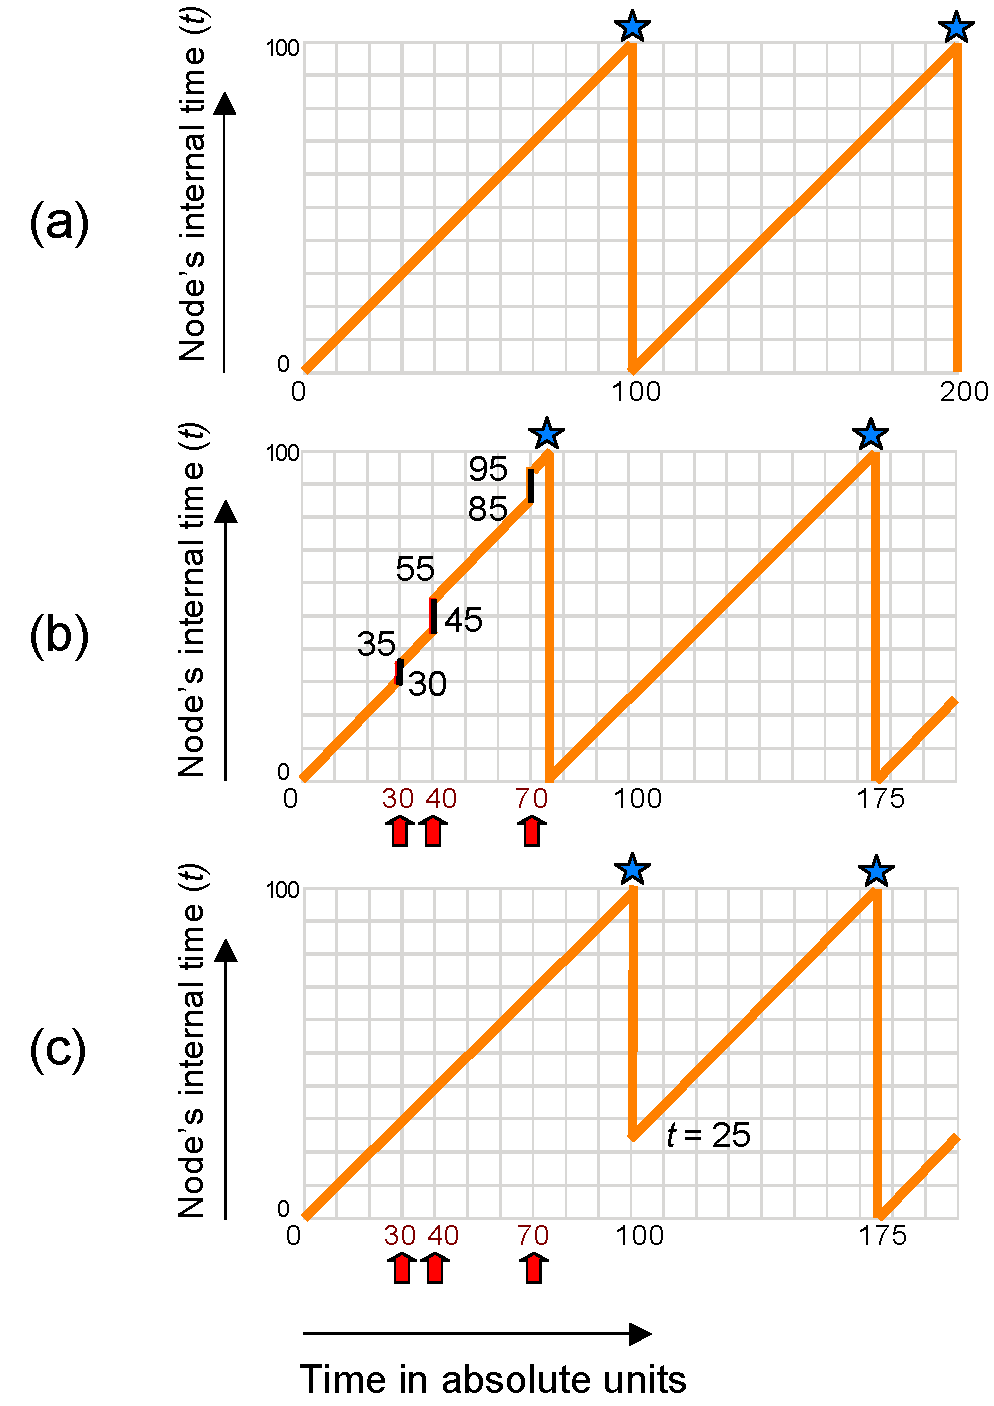
\includegraphics[width=0.8\hsize]{./figures/firing-diagram-cropped.pdf}
\end{center}
\caption{The firefly-inspired node algorithm. (a) A node fires
whenever its internal time $t$ is equal to the default time period $T$
(=100). (b) In the M\&S model, a node responds to neighbors firing
(arrows) by instantaneously incrementing $t$. (c) In RFA, a node
records the firing events and then responds all at once at the
beginning of the next cycle.}
\label{fig:firefly-example}
\end{figure}


{\bf Timestamping Messages.} In order to estimate the delay between
when a node ``fires'' and when the actual message is transmitted, we
use MAC-layer timestamping to record the MAC delay experienced by a
message prior to transmission. The MAC delay can be measured by an
event triggered by the TinyOS radio stack when the message is about to
be transmitted, and is recorded in the header of the outgoing message.
When a node receives a firing message, it uses this information to
determine the correct firing time of the transmitting node by
subtracting the MAC delay from the reception time of the message. This
is very similar to the approach used in time synchronization protocols
such as FTSP~\cite{ftsp} to estimate message transmission delays.

{\bf The {\em Reachback Response.}} The timestamping allows a node B
to correctly identify when a neighbor A fired. However it only
receives this information after some delay, and thus node B can not
react instantaneously to node A's firing.

This causes two problems. First, node B may have already fired and
thus no longer be able to react to node A. This is especially likely
for neighbor firings that occur late in a node's time
period. Furthermore, messages later in the cycle are important and
have a larger adjustment effect (as a result of $f(t)$ being concave
down). Secondly, as a result of the delays, a node may receive firing
messages {\em out of order}. The effect of applying two firing events
is not commutative. Suppose two firings occur at times $t_1$ and $t_2$
($t_1<t_2$). If a node learns of the events out of order, it will
incorrectly advance its phase by $\Delta(t_2) + \Delta(t_1)$ instead
of $\Delta(t_1) + \Delta(t_2 + \Delta(t_1))$. Therefore for the
algorithm to be correct, a node would need to undo and redo the
adjustments, quickly making the algorithm complicated and
unmanageable.

Instead, in order to deal with delayed information, we introduce the
notion of {\em reachback response.} In the reachback response, when a
node hears a neighbor fire, it does not immediately react. Instead, it
places the message in a queue, timestamped with the correct internal
time $t'$ at which the firing event occurred. When the node reaches
time $t=T$, it fires. Then it ``reaches back in time'' by looking at
the queue of messages received during the past period. Based on those
messages, it computes the overall jump and increments $t$ immediately
(Figure \ref{fig:firefly-example}(c)).

The computation is the same as in the M\&S model described in Section
\ref{sec:strogatz}; from the point of view of a node, it is as if it
were receiving firing messages instantaneously. The only difference is
that the messages it is receiving are actually from the {\em previous}
time period. Thus a node is always reacting to information that is one
time period old. In Section {\ref{sec-theory} we present theoretical
results to support why the reachback response still converges. 

%% \begin{figure}[t]
%% \begin{tabular}{lll}
%% $t_{actual}$ &  $t_{internal}$ &  $t_{internal} + {jump}$\\
%% \hline\\
%% 30 & 30 & 30 + \Delta(30) = 35\\
%% 40 & 45 & 45 + \Delta(45) = 55 \\    
%% 70 & 85 & 85 + \Delta(85) = 95 \\
%% \hline\\
%% \end{tabular}
%% \label{table:strogatz}
%% \caption{Computing the effect of neighbors firing, using the Mirollo and Strogatz Model}
%% \end{figure}


{\em Example:} Here we illustrate how the algorithm works through an
example, shown in Figure \ref{fig:firefly-example}. We first
show how the M\&S model works, i.e. when messages are received
instantaneously and the node reacts instantaneously. We then
illustrate the reachback response using the same example.

Let the time period $T = 100$ time units. Let node B start at internal
time $t=0$ and increment $t$ every unit time.  Suppose firing events
arrive at absolute times $30, 40$ and $70$. Let $\Delta(t)$ be some
jump function; here we simply pick jump values for illustration
purposes.

In the M\&S model, the node reacts as each event arrives, by causing
an instantaneous jump in its internal time. $\Delta(t)$ represents the
instantaneous jump at internal time $t$. When node B observes a
firing at time $t=30$, it computes an instantaneous jump of
$\Delta(30)=5$, and sets $t = 30+\Delta(30) = 35$. Ten more time units
from this point on it observes another event. While this event
occurred 40 units of time since the beginning of the cycle, the node
perceives it as having happened at internal time $t = 45$. The node
again computes an instantaneous jump in internal time $t=45+\Delta(45)
= 55$. After 30 more time units the node B observes another firing
event. At this point $t=85$ and the node computes an instantaneous
jump to $t=85+\Delta(85)=95$. After 5 more time units, $t=100$ and
node B fires. 

It is also possible for the computed $t$ to be larger than 100
(e.g. if $\Delta(85)=20$ then $t=85+20=105$), in which case the node
sets $t=100$, immediately fires, and resets $t=0$.

The overall effect is that node B advances its phase (or shortens
its time to fire) by 25 time units. It then continues to fire with the
default time period of $T=100$.

%% THIS IS THE TABLE DATA
%% $t_{actual}$ &  $t_{internal}$ &  $t_{internal} + {jump}$\\
%% 30 & 30 & 30 + \Delta(30) = 35\\
%% 40 & 45 & 45 + \Delta(45) = 55 \\    
%% 70 & 85 & 85 + \Delta(85) = 95 or 105\\

Now we use the same example to illustrate the reachback response. As
before, let node B start with $t=0$ and increment $t$ every time
unit. When node B receives a message, it uses the timestamping
information to determine when that message would have been received
had there been no delay. It then places this information in a queue
and continues.

When $t=100$, node B fires, resets $t=0$, and then looks at the
queue. In this example, the queue contains three events at times 30,
40 and 70. Using the same method described for M\&S, the node computes
how much it would have advanced its phase. Since all of the
information already exists, it can compute the result in one shot.  As
in the previous case, the result is that the phase is advanced by 25
time units. Node B applies this effect by instantaneously jumping from
$t=0$ to $t=25$. It then proceeds as before, firing by default at
$t=100$ if no events are received. The difference between the
reachback scheme and the original M\&S method is that the first firing
event occurs at different absolute times (100 vs 75). This influences
neighboring nodes' behavior and one must prove that the new scheme will
still converge.


%% The queue but it
%% computes using all events within the past 100 time units.  (that is
%% the previous time period). This ensures that all observed firing
%% events are processed only once.

%% \begin{verbatim}

%%              previous
%%              time period
%%           _______________
%%           |              |
%%  0             t=30     t=100    (node b's internal time)
%%  |---|-|--|---|----------|
%%  0  30 40 70  100       170      (actual time units)
%%  |____________|

%%     previous
%%     time period

%% \end{verbatim}

%% \begin{figure}[h]
%% \begin{center}
%% \includegraphics[width=1.0\hsize]{./figures/algo2.pdf}
%% \end{center}
%% \end{figure}


{\bf Pre-emptive Message Staggering.} CSMA schemes attempt to avoid
channel collisions by causing nodes to backoff for random intervals
prior to message transmission. The range of this random interval is
increased exponentially following each failed transmission attempt, up
to a maximum range.  If a small number of nodes are transmitting at
any point in time, then this approach induces low message delays.
However, if many nodes are transmitting simultaneously, delays may
become very large. CSMA works very well with bursty traffic and
non-uniform transmission times.  However, for the M\&S algorithm, the
communication pattern is very predictable and represents the worst
case for CSMA when many nodes are firing simultaneously.

In order to avoid repeated collisions and control the extent of
message delay, we explicitly add a random transmission delay to node
firing messages at the application level. We choose the delay
uniformly random between 0 and a constant $D$. In addition, after a
node fires, it waits for a grace period $W$ (where $W>D$ and $W \ll T$)
before processing the queue so that delayed messages from synchronized
nodes are received. In Section~\ref{sec-simulations}, we discuss our
choices for the parameter values and show that in practice this works
well to control message delay.

{\bf Simplified Firing Function.} In order to make the firing response
fast to compute, we chose a simple firing function $f(t) =
\ln(t)$. Using equation (\ref{eqn:strogatz}) along with
$f^{-1}(x)=e^x$, we can compute the jump in response to a firing
event, which is
$\Delta(t')=f^{-1}(f(t')+\epsilon)-t'=(e^{\epsilon}-1)t'$. To first
order $e^\epsilon = 1 + \epsilon$ (Taylor expansion), leaving us with
 a simple way to calculate the jump.

\begin{equation}\label{eqn:delta}
\Delta(t') = \epsilon t'
\end{equation}

%% RAD: There is no reason to invoke linearization
%% in fact we could have computed delta(t) exactly!!!
%% instead we use an approximation, which still isn't bad.
%%
%% Removed Text
%% In order make the firing response fast to compute, we chose a simple
%% firing function $f(t) = \ln(t)$ and we approximate $f(t)$ as being
%% linear over a small intervals. From equation \ref{eqn:strogatz}, we
%% know that $t'' = f^{-1}(f(t') + \epsilon)$. Assume that between time
%% $t'$ and $t''$, $f(t)$ can be approximated as a linear function $k't$
%% where $k'$ is the slope of $f$ evaluated at time $t'$. Thus $k' =
%% df/dt(t')$. Therefore, $t'' = (1/k') (k't' + \epsilon) = t' +
%% \epsilon/k' $.

%% If $f(t) = \ln(t)$, then its slope $k(t) = 1/t$, which makes the jump
%% extremely simple to compute: 

\subsection{Effect of Parameter Choices}
\label{sec:params}

The main parameter that affects the behavior of the system is
$\epsilon$, which determines the extent to which a node responds when
it observes a neighbor firing. A node responds to a neighbor by
incrementing its phase (shortening its time to fire) by $\epsilon t$,
where $t$ is the internal time at which the event was observed. Since
$t<T$, the maximum increment a node could make is $\epsilon T$. Thus
if $\epsilon = 1/100$, then a node can react to another node by at
most $T/100$. 

This gives us an intuitive feel for the effect of $\epsilon$, which is
made more concrete in the next section.  Choosing a larger epsilon
means that a node will take larger jumps in response to other nodes'
firing, thus achieving synchrony faster. However if $\epsilon$ is too
large, then nodes will ``overshoot'', preventing convergence. Making
$\epsilon$ small avoids overshooting but only at the cost of nodes
proceeding slowly towards convergence. In the next section we prove
that the time to synchronize is proportional to $1/\epsilon$, for
reasonable values of $\epsilon$. Later in the paper we present
simulation and testbed results that show that the system works well
over a wide range of $\epsilon$.


Other parameters such as the time period $T$ and the message
staggering delay $D$ do not affect the ability to converge, nor the
number of time periods to converge. The goal of $D$ is to stagger
messages within one broadcast neighborhood, therefore it should exceed
network density. The choice of $T$ affects overhead because it
represents the frequency with which nodes communicate --- one can
choose that to be appropriate for the application. The main constraint
is that $T \gg D$, so that there is enough time for all the messages
from a previous time period to be collected. In the face of heavy
congestion, this inequality may be violated in which case the delayed
firing events can simply be discarded.

For our implementation, we choose $T=1$sec and $D=25$ms. These
choices are somewhat arbitrary; our experimental results suggest that
the application layer delay of $25$ms works well to eliminate packet
loss during synchronized firings for neighborhoods of upto 20 nodes.


%% [SHOULD WE HAVE A SECTION ON IMPLEMENTATION DETAILS] In the
%% implementation of this algorithm for the nodes, the nodes do
%% additional tasks such as sort the queue, use a fixed size queue,
%% discard messages that are delayed beyond $T$ units of time, etc.
 	%rad
%\section{Theoretical Analysis}
\label{sec-theory}

In this section, we present an analysis of the reachback scheme for
two oscillators. Our analysis follows that of Mirollo and
Strogatz. The ideas and mathematical constructs used are similar,
though they differ in important ways that require slightly more
complex analysis.

Each oscillator is characterized by a state variable $s$ that evolves
according to $s=f(\phi)$ where $f$ is the firing function and $\phi$
is a phase variable representing where the oscillator is in its
cycle. For example, if an oscillator has finished 3/4 of its cycle,
then $\phi=3/4$. Thus $\phi\in[0,1]$ and $d\phi/dt=1/T$ where $T$ is
the period of the oscillator's cycle. We assume that the function $f$
is monotonic, increasing, and concave down. For our purposes, we
choose $f(\phi)=\ln(\phi)$.

Now consider two oscillators A and B governed by $f$. They can be
visualized as two points moving along the fixed curve $s=f(\phi)$ at a
constant horizontal velocity $1/T$, as shown in Figure
\ref{fig:theory2}. When A reaches $\phi=1$ it will fire, and B will
record the phase at which it hears A's firing. In the RFA scheme,
unlike the M\&S model, B will \emph{not} jump immediately upon hearing
A's fire; instead, B will record the time and then execute the
appropriate jump after its next firing. The jump is defined as
$\Delta(\phi)=g(f(\phi)+\epsilon)-\phi$, where $g=f^{-1}$ and
$\epsilon \ll 1$. For example, if B records $\phi_1$ as the time A
fired, when B reaches $\phi=1$ it will fire and then jump forward to
$\phi=\Delta(\phi_1)$. In the the RFA scheme, $f(\phi) = \ln(\phi)$
(and thus $g(\phi)=e^{\phi}$), therefore
$\Delta(\phi)=(e^{\epsilon}-1)\phi$. The question is whether the RFA
scheme leads to synchrony.

\begin{figure}[t]
\begin{center}
\includegraphics[width=1.0\hsize]{./figures/theory-2oscillators.pdf}
\end{center}
\caption{Two nodes A and B moving along $s=f(\phi)$}
\label{fig:theory2}
\end{figure}

\newtheorem{theorem}{Theorem}
\begin{theorem}
Two oscillators A and B, governed by RFA dynamics, will be driven to
synchrony irrespective of their initial phases.
\end{theorem}

{\bf Proof.} Consider two oscillators A and B. Consider the moment
after A has fired and jumped. In the instant after the jump, let
$\vec{\phi} = (\phi_A,\phi_B)$ denote the phases of oscillators A and
B, respectively. The {\em return map} $R(\vec{\phi})$ is defined to be
the phases of A and B immediately after the \emph{next} firing of A
(which is necessarily \emph{after} the next firing of B since A cannot
jump past B\footnote{If A fires and then jumps to $\phi_A$, then
$\phi_A \leq \phi_B$ for the following reason: If the phase of B is
$\phi_B$ when A reaches $\phi=1$, then A must have observed $B$ fire
at $\phi_x \geq 1 - \phi_B$ (since B would have fired and then taken a
positive jump). After firing A takes a jump of
$\phi_A=\Delta(\phi_x)$. $\Delta(x)$ is always $\leq 1-x$ because it
is truncated to never cause a jump past the end of the
cycle. Therefore $\phi_A \leq 1-\phi_x \leq \phi_B$.})

We now calculate the return map $R(\vec{\phi})$. Without loss of
generality assume $\phi_A < \phi_B$. Since A has just fired, B records
A's firing time as $\phi_B$. Both oscillators move forward in their
cycles until B fires. After B fires, according to our algorithm, B
jumps to phase $\Delta(\phi_B)$. In the meanwhile, A has moved forward
a distance $1-\phi_B$, reaching phase $\phi_A+1-\phi_B$, and recording
this as B's last firing time. After A's next firing, it jumps to
$\Delta(\phi_A+1-\phi_B)$, and B is at
$\Delta(\phi_B)+1-(\phi_A+1-\phi_B) =
\Delta(\phi_B)+\phi_B-\phi_A$. Substitution of the expression for
$\Delta(\phi)$ and algebraic simplification yields:

\begin{equation}\label{dynamics}
\vec{\phi}_{n+1}=R(\vec{\phi}_n)=M\vec{\phi}_n+\vec{b}
\end{equation}

Here $n$ denotes the cycle number. The vector $\vec{b}$ is defined as
  $(e^\epsilon-1,0)$, and the matrix $M$ is defined as


\begin{equation}\label{ADefn}
M=
\begin{bmatrix}
  e^\epsilon-1 & -(e^\epsilon-1) \\
  -1 & e^\epsilon \\
\end{bmatrix}
\end{equation}

%% \begin{equation}\label{bDefn}
%% \vec{b}=
%% \begin{bmatrix}
%%   e^\epsilon-1 \\
%%   0 \\
%% \end{bmatrix}
%% \end{equation}

Hence the algorithm can be described as a
linear dynamical system in $\vec{\phi}$, where $\vec{\phi} \in
[0,1] \times [0, 1]$. The unique fixed point of this dynamical
system is easily shown to be:

\begin{equation}\label{fixedPtDefn}
\vec{\phi}^*=
\begin{bmatrix}
  0 \\
  \frac{1}{2} \\
\end{bmatrix}
\end{equation}

\begin{figure}[t]
\begin{center}
\includegraphics[width=1.0\hsize]{./figures/theory-trajectory.pdf}
\end{center}
\caption{Trajectory of the oscillator phases}
\label{fig:theory1}
\end{figure}

At $\vec{\phi}^*$ both A and B would be exactly half a cycle apart. We
now show that $\vec{\phi}^*$ is unstable (i.e.. a "repeller") such that
the phases gets pushed to either (0,0) or (1,1) where the dynamics no
longer change. Introducing the change of variables
$\vec{\varphi}_n=\vec{\phi}_n-\vec{\phi}^* $ we can rewrite
(\ref{dynamics}) as

\begin{equation}\label{shiftEqn}
    \vec{\varphi}_{n+1}=M\vec{\varphi}_n
\end{equation}

By the eigendecomposition theorem, we can decompose $M$ as
$M=V\Lambda V^{-1}$, where $V$ is the matrix of composed
eigenvectors and $\Lambda$ is a diagonal matrix containing the
eigenvalues of $M$. To leading non-vanishing order in $\epsilon$,
the eigenvalues (in $\Lambda$) are $\lambda_1=\epsilon^2$ and
$\lambda_2=(1+\epsilon)$, and the principal eigendirections (the
rows of $V^{-1}$) are $\bar{v}_1=(1,1)$ and
$\bar{v}_2=(0,\epsilon)$. The decomposition allows us to rewrite
(\ref{shiftEqn}) as

\begin{equation}\label{changeOfBasisEqn}
    \vec{\theta}_{n+1}=\Lambda\vec{\theta}_{n}
\end{equation}

where $\vec{\theta}_{n}=V^{-1}\vec{\varphi}_n$ is a change-of-basis
transformation that maps all vectors into a new coordinate system
spanned by the basis $\mathcal{B}=\{\bar{v}_1, \bar{v}_2\}$. Equation
(\ref{changeOfBasisEqn}) shows us that the evolution of the system is
most simply described in terms of $\mathcal{B}$. The system's
evolution along the directions $\bar{v}_1$ and $\bar{v}_2$ is
illustrated in Figure \ref{fig:theory1}. First, all trajectories
rapidly approach the $\phi_A=0$ axis along the vector
$\bar{v}_1=(1,1)$ since $\lambda_1=\epsilon^2 \ll 1$. Upon reaching
the axis, trajectories are repelled away from $\vec{\phi}^*=(0, 1/2)$,
along the direction $\bar{v}_2=(0,\epsilon)$, since $\lambda_2 >
1$. If a trajectory approaches the axis from below $\vec{\phi}^*$, it
will slide down the axis to the state of synchrony
$\vec{\phi}=(0,0)$. Otherwise, it will climb up to $\vec{\phi}=(0,1)$,
another state of synchrony. Thus $\phi^*$ is a repeller and the
oscillators are driven to synchrony, irrespective of initial
phases. QED\\

{\bf Rate of synchronization.} How quickly the system
synchronizes depends on how fast it moves in the $\bar{v}_2$ direction
away from $\vec{\phi}^*$ before it reaches a state of synchrony. We
can estimate the time to synchronization, starting from
$\vec{\phi}^{(0)}=(\phi_A^{(0)}, \phi_B^{(0)})$. Given such an initial
state, the system's trajectory will intersect the $\phi_A=0$ axis at
approximately $\delta=\phi_B^{(0)}-\phi_A^{(0)}$. The distance from
the fixed point grows exponentially fast with eigenvalue
$\lambda_2=(1+\epsilon)$ in the $\bar{v}_2$ direction. Let $k$ denote
the number of iterations required. Solving $\lambda_2^k
(\delta-\frac{1}{2}) = \frac{1}{2}$ yields

\begin{equation}\label{rateOfSync}
    k = \frac{1}{\ln(1+\epsilon)} \ln(\frac{1}{2\delta-1}) \approx
    \frac{1}{\epsilon} \ln(\frac{1}{2\delta-1})
\end{equation}

Thus, \emph{the time to synchrony is inversely proportional to
$\epsilon$}.

\newpage

Note that these proofs are very similar to the two oscillator case for
Mirollo and Strogatz, and most likely can be extended to $n$
nodes. However extending these results to multi-hop topologies
requires considerably more sophisticated analysis
\cite{lucarelli04}. Instead we evaluate the algorithm in simulation
for different $n$ and network topologies.



 	%ankit
%\section{Evaluation Tools and Metrics}

Both our simulation and testbed experiments output a series of node
IDs and firing times. In order to discuss the accuracy of the achieved
synchronicity, it is necessary to identify groups of nodes firing
together.

For this purpose, we identify sets of node firings that fall within a
prespecified time window. We call each cluster of node firings a {\em
group}. Given a time window size $w$, the clustering algorithm outputs
a series of firing groups that meet two constraints. First, every node
firing event must fall within exactly one group.  Second, groups are
chosen to contain as many firing events as possible. 

We define the {\em group spread} as the maximum time difference
between any two firings in the group. The time window size $w$
represents the upper bound on the group spread. 

\subsection{Evaluation Metrics}

The two evaluation metrics that we are concerned with involve
the amount of time until the system achieves synchronicity (if at
all), and the accuracy of the achieved synchronicity.

\begin{description}
\item {\bf Time To Sync:} This is defined as the time that it takes
all nodes to enter into a single group and stay within that group for
9 out of the last 10 firing iterations. The value chosen for the time
window $w$ does impact the measured time to sync; a very small $w$
will result in a time to sync that is longer than with a larger $w$,
because it takes longer for all nodes to join a firing group within a
smaller time window. Also, as will be discussed in the next sections,
the simulator has lower time resolution than the testbed hardware
which means there is a limit on the accuracy it can
achieve. Therefore, for the simulator we set $w = 0.1$sec and in the
real testbed we set $w = 0.01$sec.

\item{\bf 50th and 90th Percentile Group Spread:} Recall that the
group spread measures the maximum time difference between any two
events in a firing group. We wish to characterize the {\em
distribution} of group spread for all groups after the system has
achieved synchronicity. Although synchronicity may be achieved
according to the time to sync metric above, we wish to avoid measuring
group spread while the system is still settling. Given the first sync
time $t_s$ and the time the experiment ends $t_e$, we calculate the
group spread distribution across all groups in the interval $[t_s +
\frac{(t_e - t_s)}{2}, t_e]$. In this way we are measuring the
distribution across all ``tight'' groups rather than settling
effects. We plot the 50th and 90th percentile of the distribution.

%To describe the level of
%synchronicity achieved by a given set of nodes, we proceed as follows.
%First, we examine only the time after which the system has synchronized, as
%defined by the time to sync.  To avoid penalizing systems which achieve
%tighter synchronicity than the binning parameter chosen we elide the first
%half of these spreads, thereby avoiding considering spreads produced when the
%system was still approaching its optimal level of synchronicity.  We
%calculate the 50th and 90th percentile group spread across the remaining
%data.  The meaning of these numbers is straightforward: over 50\% of the
%group firings the nodes were synchronized to at least the 50th percentile
%group spread, and likewise for the 95th percentile group spread.
\end{description}


Lastly, we define the {\em Firing Function Constant} (FFC) to be the
value $1/\epsilon$, which is the main parameter in the RFA
algorithm. As discussed in Section \ref{sec:params}, this parameter
limits the response of a node to be at most $T/FFC$ and
thus the time to synchronize is directly proportional to
$FFC$. 

\section{Simulation Results}
\label{sec-simulations}

We have implemented the Firefly algorithm in
TinyOS~\cite{tinyos-asplos00} using the TOSSIM~\cite{tossim} simulator
environment. This simulator has several limitations.  It does not
model radio delay correctly, and nor does it take into account clock
skew that occurs from variations in clock crystals in individual
wireless sensors. Despite these limitations, the simulator is useful
for exploring the parameter space of our algorithm.  This can help us
determine optimal parameter settings for the algorithm on a real
testbed as well as better understand the impact of the parameter
values on the level of synchronicity achieved. In our simulator
experiments, we explore the impact of varying:

\begin{enumerate}\addtolength{\itemsep}{-0.5\baselineskip}
\item {\bf Node topology}: \emph{all-to-all} where each node can
communicate with every other node, and a \emph{regular grid} topology
where a node can directly exchange messages with at most four other
nodes.
\item {\bf Firing function constant value}: ranging from
10-1000. Theoretically, the time to synchronize is proportional to the
firing function constant value.
\item {\bf Number of nodes {\em (n)}}: We examine whether the impact of the
firing function constant and node topology varies with the number of
nodes. The size of the all-to-all topologies is varied between 2-20
nodes with 2 node increments, and grid topologies are varied from 16,
64, to 100 nodes.
\end{enumerate}

%%% NEW FIGURES %%%

%% Percentage of synchronization for all-to-all and grid
\begin{figure*}
\begin{center}
(a)
\includegraphics[width=0.4\hsize]{./figures/mdw/ata/percent-synch.pdf}
(b)
\includegraphics[width=0.4\hsize]{./figures/mdw/grid-synch/percent-synch-grid.pdf}
\end{center}
\caption{Percentage of simulations that achieved synchronicity for
different firing function constants and numbers of nodes. (a)
All-to-all topology. Small firing function constants
(E.g. 10,20,50,150) did not achieve synchronicity most of the
time. (b) Grid Topology. Experiments with very small firing function
constants (E.g. FFC=10) or very large firing function constants
(E.g. $>500$) did not achieve synchronicity.}
\label{fig:pcnt-synch-both}
\end{figure*}

%% all-to-all time to sync and group spread
\begin{figure*}
\centering
(a)
\includegraphics[width=0.4\linewidth]{./figures/mdw/ata/tts.pdf}
(b)
\includegraphics[width=0.4\linewidth]{./figures/mdw/ata/gs-ata.pdf}
\caption{All-to-all topology. (a) Time to Sync, which for most cases
increases with increasing FFC values. (b) Group Spread. The solid bars
represent the 50th percentile spread, while the error bar indicates
the 90th percentile. For most FFC values, the group spreads remain
similar, with a slight increase as the number of nodes increases}
\label{fig:ata}
\end{figure*}

%% grid time to sync and group spread
\begin{figure*}
\begin{center}
(a)
\includegraphics[width=0.4\hsize]{./figures/mdw/grid/tts.pdf}
(b)
\includegraphics[width=0.4\hsize]{./figures/mdw/grid/gs-grid.pdf}
\end{center}
\caption{Grid Topology. (a) Time to Sync, which increases with
increasing FFC values and network diameter. (b) Group Spread. The
solid bars represent the 50th percentile spread, while the error bar
indicates the 90th percentile. Group spread remains similar over
varying FFC values, but increases with network diameter. For large
grids, FFC=500 does synchronize as well, as also shown in Figure
\ref{fig:pcnt-synch-both}.}
\label{fig:grid}
\end{figure*}

{\bf All-to-all Topology Results.}  Figures
~\ref{fig:pcnt-synch-both}(a) and \ref{fig:ata} show the results of
simulations on the all-to-all topology. We ran simulations for firing
function constant values (FFC) 10,20,50,70,100,150,300,500,750 and
1000, repeating this combination for number of nodes ranging from 2-20
in 2 node increments. For each parameter choice, we ran 10 simulations
using different random seeds to start the nodes at different
times. Each experiment was run for 3600 seconds of simulation
time. Also the time period $T=1$sec for all experiments.

Fig.~\ref{fig:pcnt-synch-both}(a) shows the percentage of simulations
that synchronized for a selection of parameter values. This percentage
represents the fraction of runs that achieved synchronicity out of the
10 total runs, for a given parameter choice of $n$ and $FFC$.  We can
see that the FFC values displayed in the figure (70,100,300,500 and
750) are fairly reliable since these cases achieved synchronicity in a
majority of the simulation runs.  Most experiments with small firing
function constants (10,20,50) did not achieve synchronicity. One
likely reason for this behavior is that small FFC values lead nodes to
make extremely large jumps, causing them to overshoot (see Section
\ref{sec:params}).

Fig.~\ref{fig:ata}(a) shows the time to synchronize as a function of
FFC value and the number of nodes. The graph shows that most FFC
constants work well. The time to sync increases with increasing FFC
value but not beyond 400 time periods. There is no clear trend with
increasing numbers of nodes, although small FFCs do not work as well
with large numbers of nodes. This is possibly because the effect of
overshoot is worsened when there are more neighbors (and thus more
total firing events per cycle to react to).

Fig.~\ref{fig:ata}(b) shows the corresponding group spreads. For most
FFC values and most $n$, the 90th percentile group spread remains the
same. The 50th percentile shows a slight increase with increasing FFCs
and a slight increase with increasing numbers of nodes. However, the
difference in the spreads is not large and thus group spreads remain
fairly similar over all parameter values. The error bars for this data
(not shown here) show that there is not much variation across
different experimental runs.

{\bf Grid Topology Results.}  Fig.~\ref{fig:pcnt-synch-both}(b) and
\ref{fig:grid} show the simulation results for regular grid topologies
of 4x4, 8x8, and 10x10 nodes. Fig. \ref{fig:pcnt-synch-both}(a) shows
the percentage of cases that synchronized for a selection of parameter
values. The results show that FFC values in the range of 20-500 almost
always achieve synchronicity in a grid topology.

The behavior of nodes in a grid topology reflects the impact of
network diameter on performance. Fig.~\ref{fig:grid} (a) shows that
large values of the firing function constant increase the time taken
to achieve synchronicity, and that this effect is more pronounced for
larger grids. Larger FFC values imply that nodes make smaller jumps
and thus converge to synchrony more slowly. For a given FFC, the time
to sync also increases slightly with network diameter, but not by much
for the smaller FFC constants. The error bars for the FFC=500
simulations (not shown here) show that there is a large variation in
time to sync and group spread across runs, most likely caused by the
initial phase distribution of nodes in the grid which can only be
corrected slowly. Barring that case, Fig.~\ref{fig:grid} (b) shows
that the group spread does not vary significantly with FFC
value. However there does seem to be an increase in spread
(i.e. decrease in accuracy) for larger grids, indicating that the
network diameter may have an impact on how well the system can
synchronize.


%%%%%%%%%%%%%%%%%%%%%%%%%%%%%%%%%%%%%%%%%%%%%%%%%%%%%%%%%%%%%%%%%%%%%%%%%%%%%%%%%%%%%%%%%%%%%%%%%%%

%\begin{figure}[p]
%\begin{center}
%\includegraphics[width=1.0\hsize]{./figures/mdw/grid/gs50.pdf}
%\includegraphics[width=1.0\hsize]{./figures/mdw/grid/gs90.pdf}
%\end{center}
%\caption{{\small {\bf The tightness of the synchronicity decreases with the number of nodes in the grid topology regardless of the number of nodes.  Furthermore, the firing function constant does not have a significant impact on the tightness of synchronicity in this topology.  These trends are retained in the 90th percentile group spread.}}}
%\label{fig:grid90}
%\end{figure}

%\begin{figure}[p]
%\begin{center}
%\includegraphics[width=1.0\hsize]{./figures/mdw/grid/gs90.pdf}
%\end{center}
%\caption{{\small {\bf 90th percentile group spread in the grid topology for different number of nodes}}}
%\label{fig:grid90}
%\end{figure}

%\begin{table}[t]
%\begin{center}
%\begin{tabular}{|c|c|c|} \hline
%Topology & Number of Nodes & Firing Function Constant \\ \hline \hline
%%all-to-all &  2  &  1000 \\
%all-to-all &  6  &  10 \\
%all-to-all &  8  &  20 \\ 
%all-to-all &  10 &  10 \\
%all-to-all &  10 &  20 \\
%all-to-all &  12 &  20 \\
%all-to-all &  12 &  50 \\
%all-to-all &  14 &  10 \\
%all-to-all &  14 &  20 \\ 
%all-to-all &  14 &  50 \\
%all-to-all &  16 &  20 \\
%all-to-all &  18 &  20 \\
%all-to-all &  20 &  20 \\ 
%grid       &  64 &  10 \\
%grid       &  64 &  750 \\
%grid       &  64 &  1000 \\
%grid       &  100 &  750 \\
%grid       &  100 &  1000 \\ \hline \hline
%\end{tabular}
%\end{center}
%\caption{{\small Cases that did not achieve synchronicity consistently across all experimental runs.}}
%\label{table:nosync}
%\end{table}

%Table ~\ref{table:nosync} shows that this occurred particularly for a firing function constant value of 20.
%As explained in section 3.4, theoretical analysis predicts that the smaller the firing function
%constant value (i.e. large $\epsilon$), the larger a node jumps in response to other nodes,
%and thus nodes should converge to synchrony faster. 


%\begin{figure}[p]
%\begin{center}
%\includegraphics[width=0.9\linewidth]{./figures/mdw/ata/gs50.pdf}
%\includegraphics[width=1.0\hsize]{./figures/mdw/ata/gs90.pdf}
%\end{center}
%\caption{{\small {\bf The tightness of synchronicity for half of the groups does not vary dramatically across different firing function constant values, but does increase with the number of nodes in an all-to-all topology.  The magnitude of the increase however is quite small.}}}
%\label{fig:ata50}
%\end{figure}

%\begin{figure}[p]
%\begin{center}
%\includegraphics[width=1.0\hsize]{./figures/mdw/ata/gs90.pdf}
%\end{center}
%%\caption{{\small {\bf 90th percentile group spread for different number of nodes in the all-to-all topology}}}
%\label{fig:ata90}
%\end{figure}



%%% OLD FIGURES %%%%

%% \begin{figure*}
%% \begin{center}
%% (a)
%% \includegraphics[width=0.4\hsize]{./figures/mdw/ata/percent-synch.pdf}
%% (b)
%% \includegraphics[width=0.4\hsize]{./figures/mdw/ata/tts.pdf}
%% \end{center}
%% \caption{All-to-all topology: (a) Percentage of simulations that
%% achieved synchronicity for different firing function constants and
%% numbers of nodes. Small firing function constants (E.g. 10,20,50,150)
%% did not achieve synchronicity most of the time. (b) For most cases,
%% the time to sync was similar over large range of FFCs.}
%% \label{fig:pcnt-synch-ata}
%% \end{figure*}

%% %% \label{fig:alltts}


%% \begin{figure*}
%% \centering
%% (a)
%% \includegraphics[width=0.4\linewidth]{./figures/mdw/ata/gs50.pdf}
%% (b)
%% \includegraphics[width=0.4\linewidth]{./figures/mdw/ata/gs90.pdf}
%% \caption{All-to-all topology: The tightness of synchronicity for the
%% groups does not vary dramatically across different firing function
%% constant values or with different number of nodes.}
%% \label{fig:ata-gs}
%% \end{figure*}

%% %% \subfigure[]
%% %%   {\framebox{\includegraphics[width=0.4\linewidth]{./figures/mdw/ata/gs50.pdf}}}
%% %% \quad\quad
%% %% \subfigure[]
%% %%   {\framebox{\includegraphics[width=0.4\linewidth]{./figures/mdw/ata/gs90.pdf}}}

%% \begin{figure*}
%% \begin{center}
%% (a)
%% \includegraphics[width=0.4\hsize]{./figures/mdw/grid-synch/percent-synch-grid.pdf}
%% (b)
%% \includegraphics[width=0.4\hsize]{./figures/mdw/grid/tts.pdf}
%% \end{center}
%% \caption{Grid Topology: (a) Experiments involving very small firing
%% function constants (E.g. FFC=10) or very large firing function
%% constants (E.g. $>500$) did not achieve synchronicity. (b) The
%% relationship between FFC and the time to synch follows the theoretical
%% predictions near-perfectly in a grid topology.}
%% \label{fig:pcnt-synch-grid}
%% \end{figure*}

%% %\label{fig:grid-tts}
%% %\end{figure}

%% \begin{figure*}
%% \centering
%% (a)
%% \includegraphics[width=0.4\linewidth]{./figures/mdw/grid/gs50.pdf}
%% (b)
%% \includegraphics[width=0.4\linewidth]{./figures/mdw/grid/gs90.pdf}
%% \caption{Grid Topology: The tightness of synchronicity decreases with
%% the number of nodes in the grid topology, while the FFC does not have
%% a sginificant impact.}
%% \label{fig:grid-gs}
%% \end{figure*}

%% %% \subfigure[]
%% %%   {\framebox{\includegraphics[width=0.4\linewidth]{./figures/mdw/grid/gs50.pdf}}}
%% %% \quad\quad
%% %% \subfigure[]
%% %%   {\framebox{\includegraphics[width=0.4\linewidth]{./figures/mdw/grid/gs90.pdf}}}


 %geetika
%\section{Wireless Sensor Network\\ Testbed Evaluation}
\label{sec-motes}

Having proven our algorithm correct in simple cases and explored the
parameter space using TOSSIM, we then tested RFA on a real sensor
network testbed. The experiments carried out on the 24-node indoor
wireless sensor network testbed, show the performance of our algorithm
running on real hardware, with a complex topology, and experiencing
communication latencies over lossy asymmetric links. The table in
Figure \ref{motelab-summary} summarizes our results, showing that RFA
can rapidly synchronize all the nodes to approx. 100 $\mu$sec.

This section is structured as follows.  First, we describe our testbed
environment, focusing on the significant ways in which the testbed
differs from the TinyOS simulator.  We then describe our use of FTSP
to provide a common global time base for nodes participating in our
experiments. We then discuss our experiments and results, and compare
them to our expectation from theory and simulation.

%% We are currently deploying 30 MicaZ sensor "motes", which consist of
%% an Atmel ATMEGA128L processor running at 7.3MHz, 128KB of read-only
%% program memory, 4KB of RAM, and a Chipcon CC2420 radio operating at
%% 2.4GHz with an indoor range of approximately 100 meters.

\subsection{Testbed Environment}

\begin{figure}
\begin{center}
\includegraphics[width=0.85\hsize]{./figures/motelab-map.png}
\end{center}
\caption{Connectivity Map: The distribution and connectivity of sensor
nodes (detailed image at {\tt http://motelab.eecs.harvard.edu/}).}
\label{connectivity-map}
\end{figure}

Our experiments ran on MoteLab~\cite{motelab-spots05-abbrv}, a
wireless sensor network testbed consisting of 24 MicaZ motes
distributed over one floor of our Computer Science and Electrical
Engineering building. The MicaZ motes have a 7.3MHz clock. Each device
is attached to a Crossbow MIB600 interface backchannel board allowing
remote reprogramming and data logging. Messages sent to the nodes'
serial ports are logged by a central server. Using this data-logging
capability, nodes report their firing times as well as information
about firing messages they observe. This information is then used to
evaluate the performance of our algorithm, as well as better
understand its behavior.

\subsubsection{Network Topology}
\label{sec-FTSP}
We conducted our experiments on the most densely populated floor, with
24 nodes. Statistics on message loss rates are calculated periodically
and tend to vary over time. Examining the connectivity map and graph
shown in Figures \ref{connectivity-map} and \ref{connectivity-graph},
one can see that this is a complex multi-hop topology. The layout of
the building produces two cliques of nodes that are connected by high
quality links (less than 20\% message loss) and these cliques are
connected by only a few bridge nodes. Further examination of the
cliques shows that a large fraction of the links are asymmetric in
quality and some nodes (e.g. 2, 26) may have no incoming links of good
quality. This type of complex topology is representative of sensor
networks distributed in a complex environment.



\begin{figure*}[t]
\begin{center}
\includegraphics[width=0.8\hsize]{figures/threshold-motelab-0200-e.pdf}
\end{center}
\caption{Connectivity graph of the nodes on our testbed showing links
with better than 80\% packet reception. This reveals two
highly-connected subgraphs and a high percentage of asymmetry in link
quality.}
\label{connectivity-graph}
\end{figure*}




\subsubsection{Time Stamping with FTSP}
\label{FTSP}

In order to evaluate the performance of RFA, we need to time stamp the
firing messages so that we can determine the accuracy with which the
firing phases align. However, this proved to be difficult in our
testbed environment. Unlike TOSSIM, our sensor nodes do not
have access to a global clock. Furthermore, since they are distributed
throughout the building, there is no single base station that can act
as a global observer and provide a common time base \cite{ftsp}. In an
ironic way, evaluating RFA requires an independent and accurate
implementation of time stamping.

%% Once a node is powered up and begins running the only clock it has
%% access to the one driven by its internal oscillator.  The crystal
%% oscillator tolerances of MicaZ and other similar wireless sensor
%% network nodes are on the order of 10 to 100 parts per million.  Over a
%% short period of time these errors prevent nodes from exchanging
%% meaningful timing information using only their local clocks.


To address this difficulty we deployed the Flooding Time
Synchronization Protocol (FTSP)~\cite{ftsp} described in Section
\ref{sec-background}. FTSP provides nodes access to a stable global
clock and allows them to time stamp events with precisions reported in
the tens of microseconds. We characterized the errors in FTSP on our
MoteLab topology in the following way. Nodes log all firing messages
they hear from other nodes and the time stamp that FTSP assigned to
them. For every firing message heard by more than two nodes, we
compute the differences between the times that FTSP reported on each
node, taking the maximum difference between any two stamps. This is
only done for messages where FTSP on both the sender and receiver
reported that the nodes were well-synchronized to the global
clock. The cumulative distribution frequency (CDF) of these errors for
all of our testbed experiments is shown in
Figure~\ref{FTSP-errors}. Note however that the FTSP errors are only
calculated for nodes that are within one hop of each other, therefore we
do not know the error in FTSP between two arbitrary nodes. Given this
caveat, our results show that FTSP can quickly synchronize nodes to
within one hop errors of tens of microseconds.

The use of FTSP as the global clock impacts our experimental results
in two ways. First, our results are pessimistic since their accuracy
is limited by the accuracy of time stamping which is likely to be in
the 5-10 $\mu$sec range. Secondly, this prevents us from making an
objective comparison of accuracy between FTSP and RFA. In the future,
we plan to use more controlled experimental setups to better evaluate
the accuracy of RFA and compare it to other methods.

\begin{figure}
\begin{center}
\includegraphics[width=0.8\hsize]{./figures/FTSPERROR.pdf}
\end{center}
\caption {CDF of one hop FTSP error rates collected during all of our
testbed experiments. FTSP provided the global clock for RFA
evaluation.}
\label{FTSP-errors}
\end{figure}


\subsubsection{Differences From the Simulator}
\label{simulator-differences}

Sensor network devices in a real environment exhibit behavior not
modeled by TOSSIM.  Most significant differences for our algorithm are
(1) communication latencies are unpredictable and difficult to measure
accurately, (2) links are asymmetric and fluctuate over time, and (3)
crystal differences cause node clocks to tick at different rates. All
these effects make it difficult for a node to know exactly when
another node fired, and unlikely that it will hear every firing
message sent by its neighbors.

Paradoxically, our testbed is {\em better} than TOSSIM in one very
significant way. The sensor node hardware has a high-precision clock
and high-precision timer components. A TinyOS component written for
our project allows nodes to both locally time stamp and set timers at
$\mu$sec level resolution by multiplexing the {\tt SysTime} and {\tt
MicroTimer} components onto one hardware counter. The simulator TOSSIM
provides 4MHz local time stamping through access to its internal
clock, but no equivalent of the {\tt MicroTimer} component, forcing us
to rely on the standard TinyOS {\tt Timer} component with its
millisecond resolution. This limits the resolution of the jumps a node
can take and therefore the algorithm achieves only millisecond
accuracy in simulation. As we were using the simulator primarily to
explore the impact of parameter and topology, we felt the lack of
precision this introduced was acceptable.  The higher frequency {\tt
MicroTimer} component is the primary reason that group spread results
from our testbed experiments are much better than the simulation,
which at first would seem surprising.

\subsection{Performance Evaluation} 

\label{performance-evaluation}


The table in Figure \ref{motelab-summary} summarizes the results from
our experiments. We conducted four experiments with firing function
constants (FFC) 100, 250, 500 1000.

In each of these experiments the network achieves synchronicity. In
the case with a FFC of 100, the network is synchronized within 5
minutes, with a group spread of 131 $\mu$sec. As expected from our
theoretical and simulation studies, the time to synchronize increases
with larger firing function constants. The table also shows the 50th
and 90th percentile group spread, and Figure \ref{groupspread-cdf}
plots the group spread CDFs for each of the four FFCs. As we can see
they are striking similar, aligning with our expectations from theory
and simulations that group spread does not depend on the FFC value.

These results are very encouraging, given the caveats on our time
stamping and the complexity of the testbed environment. However, there
are also several features which are still unexplained and we plan to
investigate these more in the future. Here we discuss two examples.

One observation from the CDF plot in Figure \ref{groupspread-cdf} is
that there seems to be a limit on the achievable group spread of
around 100 $\mu$sec.  This could be related to FTSP accuracy, but it
is also affected by clock skew. We expect clock skew to impact the
accuracy of RFA because the M\&S model upon which it is based assumes
that nodes agree on a fixed firing period. However, two perfectly
synchronized nodes will diverge on the very next firing by the amount
of drift that exists in their clocks --- introducing an error that is on
the order of the crystal accuracy. This causes the nodes to constantly
readjust their phases. Clock skew also impacts the accuracy indirectly
when nodes use the message delay (measured by the sender's clock) to
adjust their own phase. In the future we plan to investigate the
effects of clock skew more rigorously and look at alternate models of
synchronization, such as synchronized clapping, where both frequency
and phase are adjusted.

%% note clock skew is 1-100 parts per million, for a ~8MHz clock this is
%% at most 100/8 ~ 10usec

\begin{figure}[t]
\begin{center}
\begin{small}
\begin{tabular}{|lllll|} \hline
{\em FFC constant} & 
{\em Time to} & 
{\em 50th pct} &
{\em 90th pct} &
{\em Mean group} \\
{\em } &
{\em sync (sec)} &
{\em spread} & 
{\em spread} & 
{\em std dev} \\
&
&
{\em ($\mu$sec)} & 
{\em ($\mu$sec)} & 
\\
\hline
100 & 284.3 & 131.0 & 4664.0 & 410.4 \\
250 & 343.6 & 128.0 & 3605.0 & 572.2 \\
500 & 678.1 & 154.0 & 30236.0 & 1327.8 \\
1000 & 1164.4 & 132.0 & 193.0 & 63.6 \\
\hline
\end{tabular}
\end{small}
\end{center}
\caption{Summary of Testbed Results. Four experiments were run on the
24 node testbed, with different firing function constants (where $FFC
= 1/\epsilon$) As expected, the time to synchronize increases with
FFC. The 50th percentile group spread is similar for all four
experiments.}
\label{motelab-summary}
\end{figure}

\begin{figure}
\begin{center}
\includegraphics[width=0.8\hsize]{./figures/CDFTOT.pdf} 
\end{center} 
\caption{CDF of RFA Group Spread. The four different firing function
constants in the testbed experiments produce similar levels of
synchronicity.}
\label{groupspread-cdf} 
\end{figure} 

%% This was completely bogus! and caught by the reviewers.
%% the theory and simulation suggest the OPPOSITE!
%% \caption{CDF of RFA Group Spread: The four different firing function
%% constants in the testbed experiments produce remarkably similar levels
%% of synchronicity. Our simulator and theoretical results indicate that the
%% tightness achieved should scale with the firing function constant chose, and
%% so these results are somewhat confusing.  However, we do achieve good
%% synchronicity across all four firing function constants.


A second observation arises from looking at the group spread over
time. We observed that even after tight groups form, occasionally
disturbances still occur during the experiment. We refer to these as
{\em dispersive events}. Figure \ref{phaseplot-motelab-specific} (a)
shows an example of a dispersive event where the nodes fall out of
phase and the system recovers from this impulse over the next few
firing periods. Figure \ref{phaseplot-motelab-specific} (b) shows a
different time course with the occurrence of two dispersive events
which cause the group to spread over approximately 0.1 $sec$
range. Note that these dispersive events are included in the data in
Table ~\ref{motelab-summary} and impact the 90th percentile group
spread. Analysis of the information collected during this experiment
showed no clear reason for this spurious firing. It is unlikely to be
caused by the algorithm, since the extent of dispersion is larger than
the maximum jump possible given the FFC. What is encouraging is that
the recovery from the 100 msec range dispersive events takes only a
few rounds to achieve, thus showing that the system can recover
quickly from perturbation. However, a more rigorous instrumentation
and experimentation setup will be required to pinpoint the causes
behind this behavior.

\begin{figure*}[t]
\begin{center}
(a)
\includegraphics[width=0.4\hsize]{./figures/GROUPDYNAMICS-SPECIFIC.pdf}
(b)
\includegraphics[width=0.4\hsize]{./figures/PHASEPLOT-SPECIFIC.pdf}
\end{center}
\caption{Dispersive events (a) This plot shows the group dynamics for
several firing periods following the effect of one node falling out of
sync. Nodes offsets against the average group firing time are plotted
with respect to time. (b) This plot shows a different example, with
FFC=1000. After the system has stabilized there are still two cases
where nodes jump out of phase and are re-incorporated into the group.}
\label{phaseplot-motelab-specific}
\end{figure*}


%% RAD
%%
%% I removed these because it is not clear to me the either of these
%% are potential explanations for the dispersive events. One should
%% be able to validate/substantiate these ideas by looking at the actual data.
%% the long-lost nbrs doesn't make sense since all of the nodes are tightly
%% clustered so even if you heard a long lost neighbor, the correction could never
%% be that large. Unless th message delay time was garbled....

%% what puzzles me the most is that the dispersion is huge, maybe even too large
%% given the FFC which limits the amount of corrective action possible in one
%% step - so it seems more as if the nodes somehow took a big hiccup somewhere
%% Given the our experinec with the counter roll-over problems like in simulation
%% seems premature to spend this much time discussing possible issues

%% Actually, to substantiate my argument
%% In the figure X, with FFC=1000
%% a dispersive event is approximate 0.1 sec in height.
%% With the FFC constant, a node could move only .001sec at most in one cycle.
%%

%%%%%%
%% \begin{itemize}
%% \item {\bf Clock Skew:} The error associated between any two clocks
%% acts as a constant dispersive force limiting the accuracy of our
%% algorithm.  Based on their interactions, all nodes may attempt to
%% choose a next firing time that is perfectly aligned. Because of clock
%% skew they will end up distributed with a spread dependent on the
%% accuracy of the crystals used to drive their hardware counters.

%% Clock skew also impacts the timing of radio events.  The delay to send a
%% message is measured by the sender and applied by the receiver.  Differences
%% between node clocks will cause an error when the receiver applies this delay
%% to calculate when the sender fired in its local time frame.

%% \item {\bf Long-lost Neighbors:} Lossy links can cause a node to suddenly
%% hear from another node that it has not heard from for a long time, again
%% precipitating a large correction.
%% \end{itemize}


%% RAD I took out this graph since it was adding much to the text or 
%% the other two dispersive event pictures which are much more informative
%% \begin{figure}[p]
%% \begin{center}
%% \includegraphics[width=0.8\hsize]{./figures/PHASEPLOT.pdf}
%% \end{center}
%% \caption {\small {\bf Phase Portrait for 1000 Firing Function Constant.}
%% {\em
%% This plot shows a phase portrait for a testbed experiment with a firing
%% function constant of 1000 exhibiting a striking display of node capture.
%% Node 18 is the last node to join the group and the phase portrait shows it
%% racing around to catch the existing group.  As it draws closer the period of
%% the larger group relaxes as it is less and less influenced by the outlier. 
%% }}
%% \label{phaseplot-motelab}
%% \end{figure}

 	%gwa
%\section{Comparison to Other Methods}

Compared to algorithms such as RBS, TPSN and FTSP\cite{rbs,ftsp,tpsn},
the firefly-inspired algorithm represents a radically different
approach. All of the nodes behave in a simple and identical
manner. There are no special nodes, such as the root in TPSN or
reference node in RBS, that need to elected. A node does not maintain
any per-neighbor or per-link state; in fact it is completely agnostic
to the identity of its neighbors. The algorithm remains the same even
if the topology is multi-hop. There are no network-level
datastructures, such as the spanning tree in TPSN, that must be
re-established in case of topology change. As a result of these
properties, the algorithm is {\em implicitly robust to the
disappearance of nodes and links}. Lucarelli et al \cite{lucarelli04}
have shown that the algorithm works on time-varying topologies; our
testbed results show that the algorithm performs well even with
asymmetric, lossy links. The inherent adaptive nature of such
algorithms is one of the main attractions of biologically-inspired
approaches.

%% The goal of this paper was to determine whether such algorithms, based
%% on simple distributed control principles, were feasible in a the
%% wireless sensor network arena.

Nevertheless, it is not yet clear whether such an algorithm will be
competitive to algorithms such as TPSN and FTSP, in terms of accuracy
and overhead, and much work remains to be done. In terms of accuracy,
RFA achieves ~100 $\mu$sec which is significantly less than the
reported 10 $\mu$sec accuracy of FTSP, although as discussed before it
is difficult to make a clear comparison because of the errors caused
by using FTSP as our evaluation clock. We believe that the accuracy
can be increased to tens of microseconds by eliminating errors in our
evaluation methodology and by using a better optimized MAC-layer delay
estimation (as used in FTSP \cite{ftsp}).  However beyond that, the
accuracy will still be limited by clock skew, as discussed in Section
\ref{performance-evaluation}. We intend to investigate models that
synchronize both phase and frequency, which would eliminate errors
cause by clock skew. A second shortcoming of RFA is that the
communication overhead is high. In particular, we choose $T=1$ sec,
unlike FTSP which has a time period of 30 seconds. Assuming one could
compensate for clock skew, the main limit on $T$ is the time taken to
synchronize from startup. RFA takes approximately 200 time periods to
synchronize on MoteLab, which is significantly more than the diameter
of the network. On the other hand, the system recovers quickly from
small dispersive events. One option would be to use a simple
mechanism, such as an initial flood, to bring all nodes to within a
small phase difference quickly. Then RFA could operate at a much lower
frequency to tighten the accuracy and maintain synchronicity. A
different option is to allow nodes to asynchronously backoff, or
increase, their time period in multiples of $T$ depending on whether
they observe many out-of-phase firing events in their
neighborhood. Thus nodes would self-adjust the overhead.


%% Besides the above limitations, our algorithm also has some other
%% unique challenges, especially in terms of analysis. While the
%% algorithm is exceedingly simple, the analysis of its effect in a
%% distributed setting is not. Sophisticated mathematics is required to
%% prove convergence in a network \cite{lucarelli04} and it is difficult
%% to specify simple back-of-the envelop calculations on multi-hop
%% convergence time. Nevertheless, the inherent fault-tolerant and
%% adaptive quality of the algorithm is very attractive, and in that
%% respect it shares many characteristics with well-established
%% algorithms such as Ethernet/CSMA that are also based on simple node
%% adaptation strategies.



%% However, a much more difficult source of error is the
%% constant error introduced by clock skew. The nodes assume a default
%% fixed frequency, however because of clock skew their actual time
%% periods may differ by as much as .1 msec. Thus even if two nodes
%% completely agree on the phase, in the next time period they will fire
%% at different times. This causes the algorithm to constantly be
%% adjusting and in the end the effective frequency is in fact lower than
%% 1 sec. This lack of true agreement on frequency adds a constant error
%% to the process, and it is suggestive that our current accuracy of 100
%% microseconds is comparable to the expected skew on the clocks. One
%% approach to compensate would be to use models of distributed
%% synchronization that synchronize both phase and frequency - such as
%% models of how humans synchronize clapping [cite].

\section{Conclusions and Future Work}

In this paper we have presented a decentralized algorithm for
synchronicity, based on a mathematical model of synchronicity achieved
by biological systems. Our results show that even though the
theoretical models make simplifying assumptions, this technique still
works well and robustly in the face of realistic radio effects and
hardware limitations. In particular, we modified the algorithm to deal
with communication latencies, but it still achieved synchronicity
reliably and showed predictable behavior in relation to parameter
choice. In the future we intend to study in detail how lossy links,
clock skew and topology parameters affect the model. A detailed study
of the robustness of the system will also help us better understand
whether the adaptive and robust behavior of biological systems can be
leveraged to design robust algorithms for sensor networks.

\section{Acknowledgements}

Nagpal is supported by a Microsoft Faculty Fellowship, Patel is
supported by a NSF graduate Fellowship. We also thank Uri Braun, who
worked on initial stages of the project.
 %all

%%%%%%%%%%%%%  THIS IS WHERE THE BIBLIOGRAPHY GOES %%%%%%%%%

\def\baselinestretch{0.92}
\begin{footnotesize}
\setlength{\itemsep}{2in}
\bibliographystyle{abbrv} \bibliography{sensys}
\end{footnotesize}

\end{document}
